\chapter{Metodologia}
\label{chap:metodologia}

\section{Estimativa das componentes e da amplitude do campo magnético}
\label{sec:componentes_campo}

Na seção \ref{sec:Gauss-Ampere}, mostrei que, se uma camada equivalente plana 
com direção de magnetização uniforme e arbitrária 
reproduz uma determinada componente $B_{\alpha}(x, y, z)$ (equação \ref{eq:B-alpha-true-generic}),
$\alpha = x, y, z$, do campo de indução magnética $\mathbf{B}(x, y, z)$ (equação \ref{eq:B-true-generic}) 
produzido por um conjunto de fontes magnéticas arbitrárias, esta camada deve, 
obrigatoriamente, reproduzir as demais componentes do campo $\mathbf{B}(x, y, z)$.
Nesta seção, apresento um método para estimar as componentes e a amplitude do campo de indução 
magnética de um conjunto de fontes magnéticas a partir da inversão de dados de uma determinada 
componente.

\subsection{Parametrização e problema direto}
\label{subsec:balpha_prob_dir}

Considere uma camada equivalente plana localizada em $z = z_{c}$, que possui uma distribuição 
contínua de intensidades de momento magnético $p(x'',y'',z_{c})$ e uma direção de magnetização 
arbitrária $\hat{\mathbf{u}}(I, D)$ (equação \ref{eq:B-alpha-layer}). 
Em situações práticas, não é possível determinar esta distribuição contínua de intensidade de momentos 
sobre a camada equivalente. 
Por esta razão, a camada é aproximada por um conjunto discreto de $M$ dipolos (fontes equivalentes) 
localizados no plano $z = z_{c}$ (Figura \ref{fig:eqlayer_balpha_sketch}).
A componente $\alpha$, $\alpha = x, y, z$, do campo de indução magnética produzida por esta camada 
discreta (componente $\alpha$ predita) no ponto $(x_{i},y_{i},z_{i})$, $i=1,\dots,N$, é dada por 
\begin{equation}
B^{\alpha}_{i} (\mathbf{p})  = \mathbf{g}^{\alpha}_{i}(\mathbf{q})^{\top} \, \mathbf{p},
\label{eq:B-alpha-pred-i}
\end{equation}
em que $\mathbf{q}$ é um vetor $2 \times 1$ (vetor de direção de magnetização) definido 
em termos da inclinação e declinação ($I$ e $D$) da magnetização total na camada equivalente
\begin{equation}
\mathbf{q} = \begin{bmatrix}
I \\ D 
\end{bmatrix} \: ,
\label{eq:q-vector}
\end{equation}
$\mathbf{p}$ é um vetor $M \times 1$ (vetor de momentos magnéticos) cujo $j$-ésimo elemento, $j=1,\dots,M$, 
é a intensidade do momento magnético $p_{j}$ (em $A \, m^{2}$) do $j$-ésimo dipolo e 
$\mathbf{g}^{\alpha}_{i}(\mathbf{q})$ é outro vetor $M \times 1$ cujo $j$-ésimo elemento é definido pela 
função harmônica 
\begin{equation}
g_{ij}^{\alpha}(\mathbf{q})  = \gamma_{m} \, {\mathbf{M}^{\alpha}_{ij}}^{\top} \, \hat{\mathbf{u}}(\mathbf{q}) \: .
\label{eq:g_ij-alpha}
\end{equation}
Nesta equação, $\hat{\mathbf{u}}(\mathbf{q}) \equiv \hat{\mathbf{u}}(I, D)$ é um vetor unitário
definido pela equação \ref{eq:u-hat} em função da inclinação e declinação 
da magnetização na camada equivalente ($I$ e $D$) e $\mathbf{M}^{\alpha}_{ij}$ é um vetor $3 \times 1$ 
dado por 
\begin{equation}
\mathbf{M}^{\alpha}_{ij} = \begin{bmatrix}
\partial_{\alpha x} \frac{1}{r''} \\
\partial_{\alpha y} \frac{1}{r''} \\
\partial_{\alpha z} \frac{1}{r''}
\end{bmatrix} \quad ,
\label{eq:Mij-matrix-alpha}
\end{equation}
em que $\partial_{\alpha\beta} \frac{1}{r''} \equiv \frac{\partial^{2}}{\partial \alpha \partial \beta} \frac{1}{r''}$ 
representa a segunda derivada da função $\frac{1}{r''}$ (equação \ref{eq:inv-r''}) em relação a $\alpha$ e $\beta$, 
$\alpha = x, y, z$, $\beta = x, y, z$, avaliada nas coordenadas $(x, y, z) = (x_{i}, y_{i}, z_{i})$ do $i$-ésimo dado  
observado e $(x'', y'', z_{c}) = (x_{j}, y_{j}, z_{c})$ da $j$-ésima fonte equivalente.
A componente $\alpha$ predita $B^{\alpha}_{i} (\mathbf{p})$ (equação \ref{eq:B-alpha-pred-i}) é 
obtida a partir da discretização da integral que define a componente $\tilde{B}_{\alpha}(x, y, z)$
(equação \ref{eq:B-alpha-layer}) produzida pela camada equivalente contínua.
Note que $B^{\alpha}_{i}(\mathbf{p})$ possui uma relação linear com o vetor de momentos 
magnéticos $\mathbf{p}$.

%% Figura
\begin{figure}[H]
	\centering
	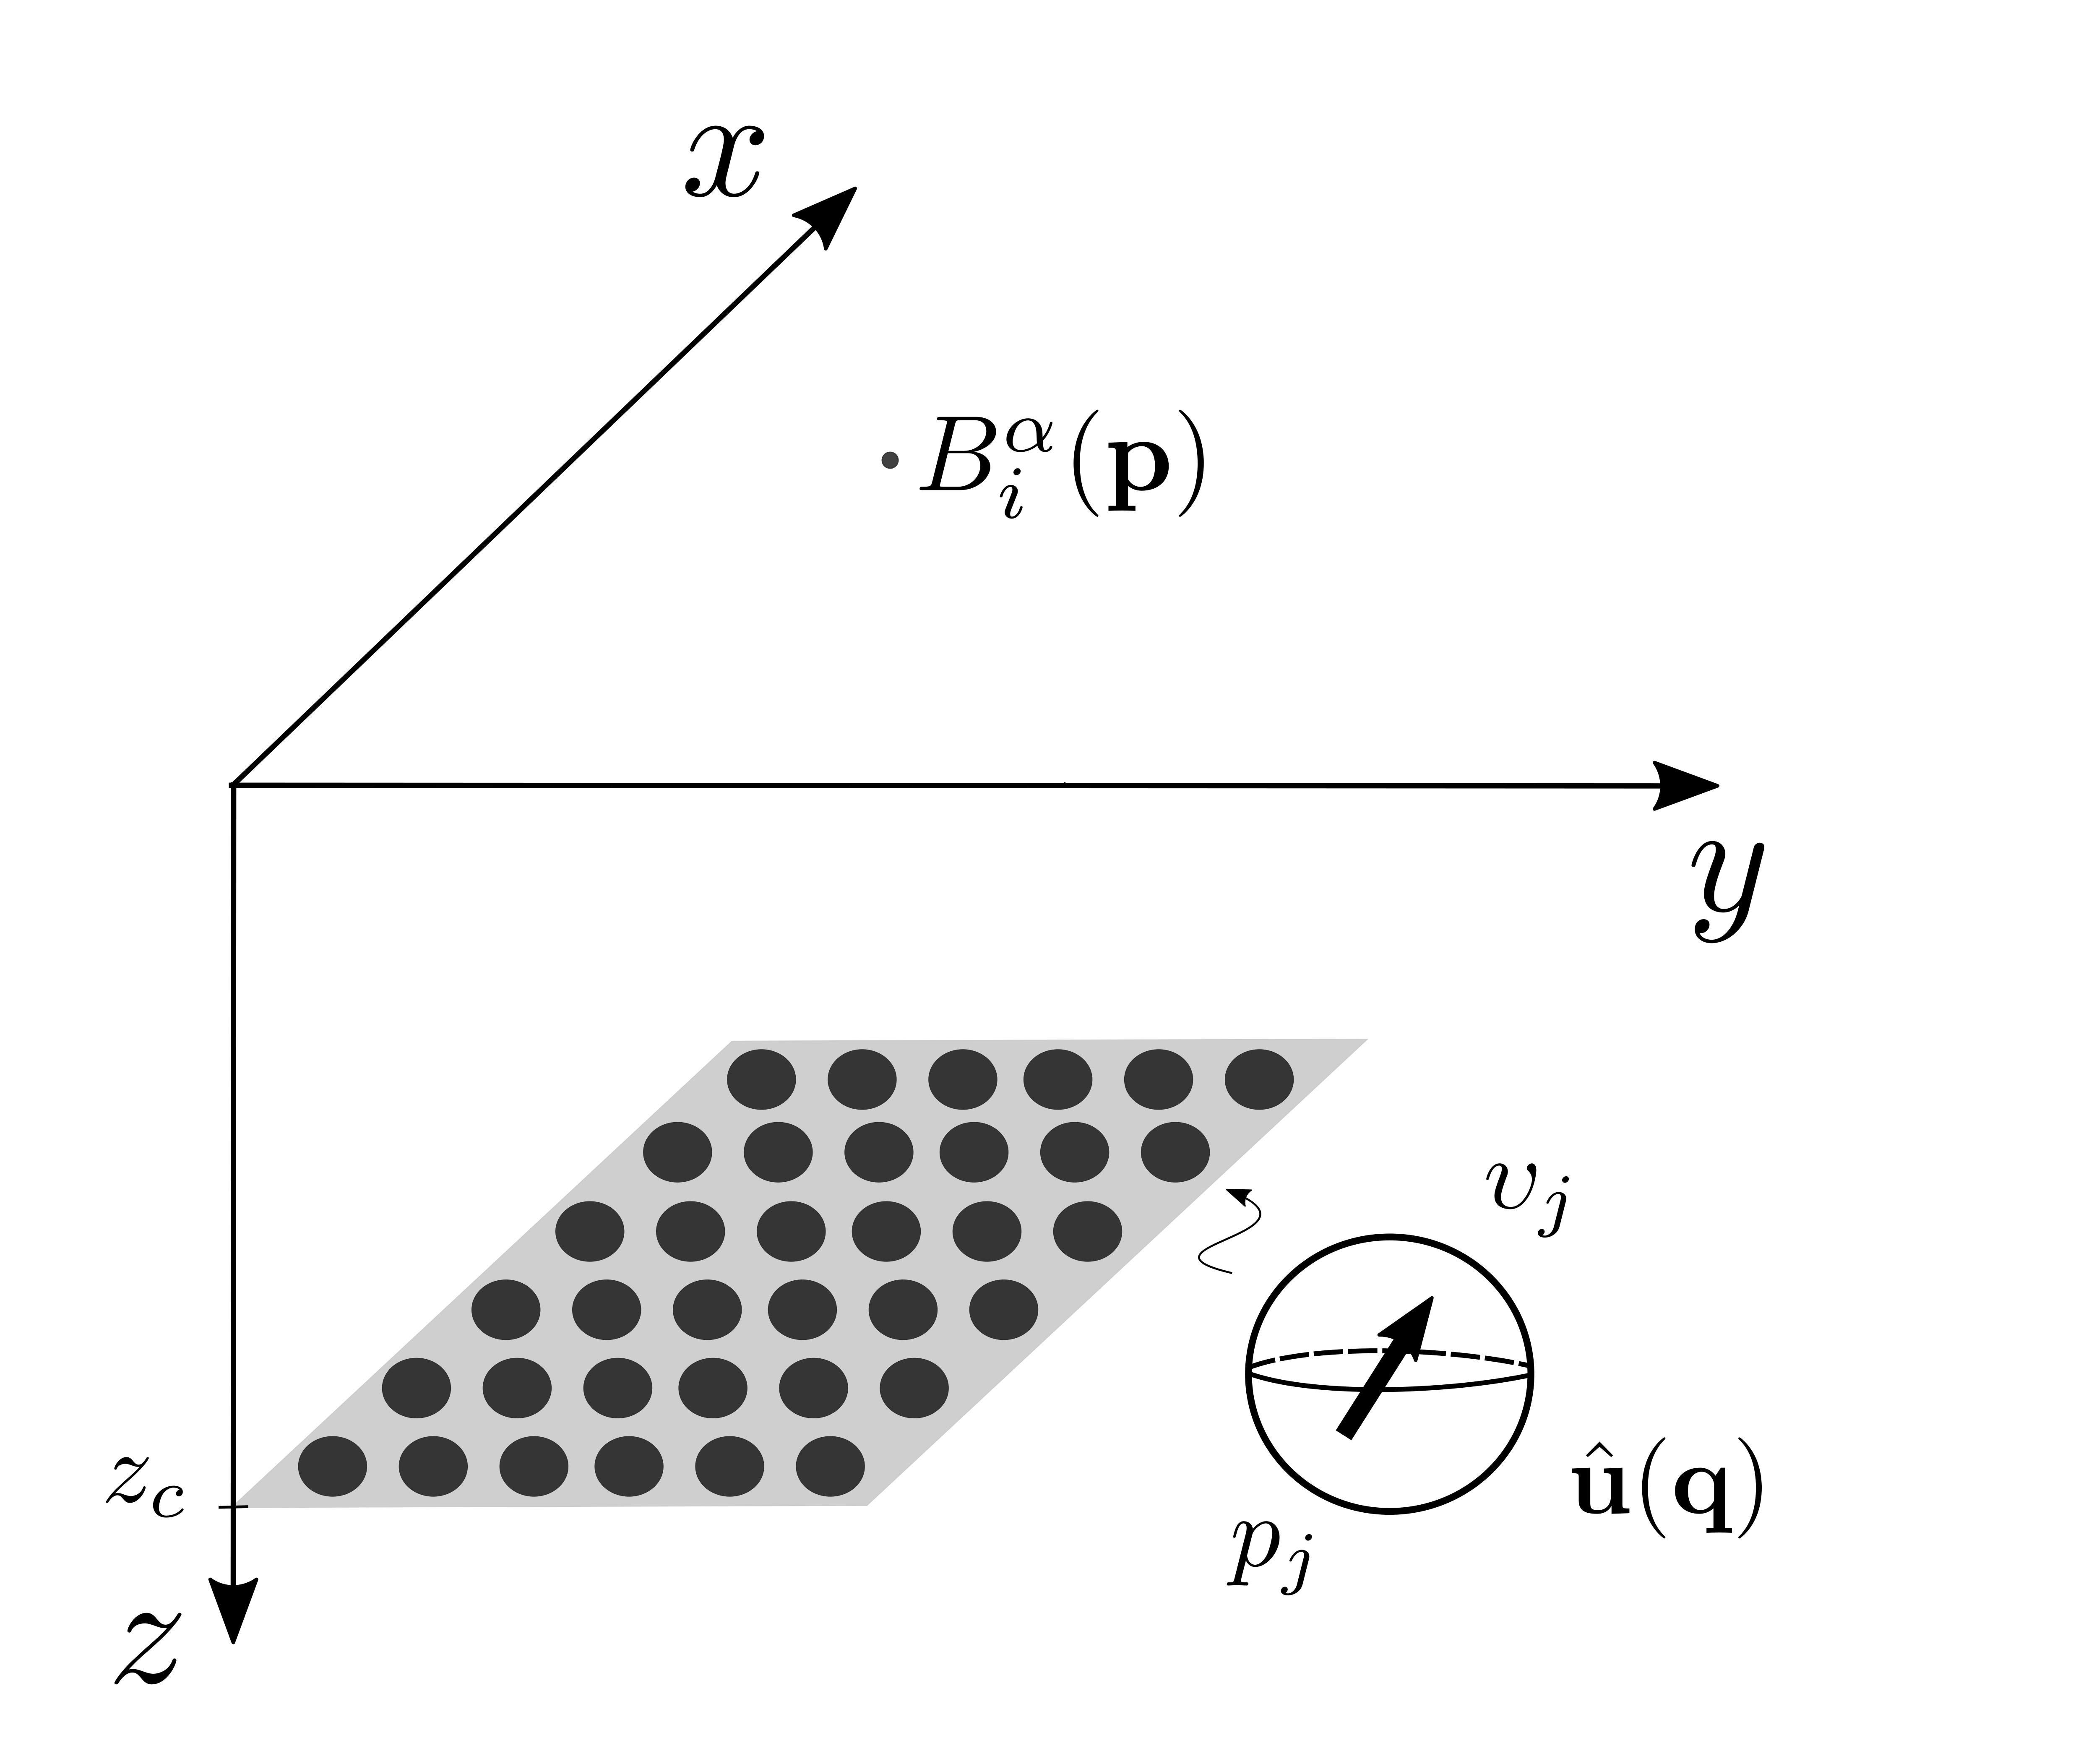
\includegraphics[width=.7\textwidth]{Fig/mag_vec/eqlayer_figure_balpha.png}
	\caption{Representação esquemática da camada equivalente para a componente $\alpha$ do campo de 
	indução magnética. A camada é posicionada sobre o plano horizontal $z = z_{c}$. 
	$B^{\alpha}_{i}(\mathbf{p})$ é a componente $\alpha$ predita (equação \ref{eq:B-alpha-pred-i}) no 
	ponto $(x_{i},y_{i},z_{i})$ pelo conjunto de $M$ fontes equivalentes (pontos pretos). 
	Cada fonte é localizada em um ponto  $(x_{j},y_{j},z_{c})$, 
	$j = 1,\dots, M$, e é representada por um dipolo de volume unitário $\upsilon_{j}$ 
	com direção de magnetização $\hat{\mathbf{u}}(\mathbf{q})$ e momento magnético $p_{j}$.}
	\label{fig:eqlayer_balpha_sketch}
\end{figure}

\subsection{Problema inverso}
\label{subsec:balpha_prob_inv}

Seja $\mathbf{B}^{\alpha}_{o}$ o vetor de dados observados cujo $i$-ésimo elemento é a componente 
$\alpha$, $\alpha = x, y, z$, do campo magnético produzida por fontes magnéticas arbitrárias no ponto 
$(x_{i},y_{i},z_{i})$, $i = 1, \dots, N$. Similarmente, seja $\mathbf{B}^{\alpha}(\mathbf{p})$ 
o vetor de dados preditos cujo $i$-ésimo elemento é a componente $\alpha$ predita 
$B^{\alpha}_{i} (\mathbf{p})$ (equação \ref{eq:B-alpha-pred-i}) produzida por uma camada equivalente 
discreta no mesmo ponto $(x_{i},y_{i},z_{i})$. 
Para estimar o vetor de momentos magnéticos $\mathbf{p}$ que minimiza a diferença entre 
$\mathbf{B}^{\alpha}_{o}$ e $\mathbf{B}^{\alpha}(\mathbf{p})$, minimizo a seguinte função 
objetivo
\begin{equation}
\Psi(\mathbf{p}) =\lVert \mathbf{B}^{\alpha}_{o} - \mathbf{B}^{\alpha}(\mathbf{p}) 
\rVert_{2}^{2} + \, \mu  \parallel \mathbf{p} \parallel_{2}^{2} \: ,
\label{eq:goal_function_vec}
\end{equation}
em que o primeiro e o segundo termo da equação \ref{eq:goal_function_vec} são a função de ajuste e a 
função regularizadora de Tikhonov de ordem zero, $\mu$ é o parâmetro de regularização e 
$\| \cdot \|_{2}^{2}$ representa o quadrado da norma Euclidiana. 
Usando uma direção de magnetização $\hat{\mathbf{u}}(\mathbf{q})$ (equação \ref{eq:g_ij-alpha}) arbitrária,
a minimização da função objetivo $\Psi(\mathbf{p})$ (equação \ref{eq:goal_function_vec}) resulta no 
sistema linear abaixo:
\begin{equation}
\left[ {\mathbf{G}^{\alpha}}^{\top} \mathbf{G}^{\alpha} + \mu \, \mathbf{I} \right] 
\bar{\mathbf{p}} = {\mathbf{G}^{\alpha}}^{\top} \mathbf{B}^{\alpha}_{o} \: ,
\label{eq:linear_sys_p_alpha}
\end{equation}
em que $\mathbf{G}^{\alpha}$ é uma matriz de dimensão $N \times M$ cujo elemento $ij$ é dado pela função 
harmônica $g_{ij}^{\alpha}(\mathbf{q})$ (equação \ref{eq:g_ij-alpha}), avaliada para um vetor de direção 
de magnetização $\mathbf{q}$ (equação \ref{eq:q-vector}) arbitrário, e $\mathbf{I}$ é a matriz identidade 
de ordem $M$. Usando a distribuição de momentos magnéticos $\bar{\mathbf{p}}$ estimada pelo 
sistema linear \ref{eq:linear_sys_p_alpha}, as outras componentes do campo magnético predito pela 
camada equivalente são calculadas escolhendo-se os $\alpha$ correspondentes nas equações 
\ref{eq:B-alpha-pred-i} -- \ref{eq:Mij-matrix-alpha}. 
Por fim, usando as três componentes $B^{\alpha}_{i}(\bar{\mathbf{p}})$
(equação \ref{eq:B-alpha-pred-i}), $\alpha = x, y, z$, calculo a amplitude do campo de indução 
magnética produzido pela camada equivalente discreta em cada ponto $ (x_{i}, y_{i}, z_{i}) $, 
$i = 1, \dots, N$, da seguinte forma:
\begin{equation}
B_{i}(\bar{\mathbf{p}}) = \sqrt{[B^{x}_{i}(\bar{\mathbf{p}})]^{2} + 
[B^{y}_{i}(\bar{\mathbf{p}})]^{2} + [B^{z}_{i}(\bar{\mathbf{p}})]^{2}} \: .
\label{eq:amplitude_field}
\end{equation}

\section{Estimativa da direção de magnetização}
\label{sec:mag_dir_est}

Na seção \ref{sec:distribuicao-positiva}, mostrei que, para uma camada equivalente plana 
reproduzir a anomalia de campo total $\Delta T(x, y, z)$ (equação \ref{eq:Delta-T-true-mag-uniform}) 
produzida por um conjunto de fontes magnéticas com direção de magnetização uniforme, a sua distribuição 
de intensidades de momento magnético $p(x'', y'', z_{c})$ 
deve ser toda positiva (equação \ref{eq:positivity_prop}). Nesta seção, apresento um método 
iterativo que usa este vínculo de positividade dos momentos magnéticos para estimar a direção de 
magnetização uniforme das fontes magnéticas a partir da inversão de dados de anomalia de campo total.

\subsection{Parametrização e problema direto}
\label{subsec:mag_dir_prob_dir}

Considere uma camada equivalente plana localizada em $z = z_{c}$, que possui uma distribuição 
contínua de intensidades de momento magnético $p(x'',y'',z_{c})$ (equação \ref{eq:B-alpha-layer}). 
Em situações práticas, não é possível determinar esta distribuição contínua sobre a camada equivalente. 
Por esta razão, a camada é aproximada por um conjunto discreto de $M$ dipolos (fontes equivalentes) 
localizados no plano $z = z_{c}$ (Figura \ref{fig:eqlayer_tfa_sketch}). 
A anomalia de campo total produzida por esta camada 
discreta (anomalia de campo total predita) no ponto $(x_{i},y_{i},z_{i})$, $i=1,\dots,N$, é dada por 
\begin{equation}
\Delta T_{i}(\mathbf{s}) = \mathbf{g}_{i}(\mathbf{q})^{\top} \mathbf{p},
\label{eq:tfa-pred-i}
\end{equation}
em que $\mathbf{s}$ é um vetor $(M + 2) \times 1$ particionado dado por 
\begin{equation}
      \mathbf{s} = \begin{bmatrix}
		\mathbf{p} \\
		\mathbf{q}
	\end{bmatrix} \: ,
	\label{eq:s-vector}
\end{equation}
$\mathbf{q}$ é o vetor de direção de magnetização (equação \ref{eq:q-vector}), 
$\mathbf{p}$ é um vetor $M \times 1$ (vetor de momentos magnéticos) cujo $j$-ésimo elemento, $j=1,\dots,M$, 
é a intensidade do momento magnético $p_{j}$ (em $A \, m^{2}$) do $j$-ésimo dipolo e 
$\mathbf{g}_{i} (\mathbf{q})$ é outro vetor $M \times 1$ cujo $j$-ésimo elemento é definido pela 
função harmônica 
\begin{equation}
g_{ij} (\mathbf{q})  = \gamma_{m} \hat{\mathbf{u}}_{0}^T \, 
\mathbf{M}_{ij} \, \hat{\mathbf{u}}(\mathbf{q}) \: .
\label{eq:g_ij}
\end{equation}
Nesta equação, $\hat{\mathbf{u}}_{0} \equiv \hat{\mathbf{u}}(I_{0}, D_{0})$ e 
$\hat{\mathbf{u}}(\mathbf{q}) \equiv \hat{\mathbf{u}}(I, D)$ são vetores unitários
definidos pela equação \ref{eq:u-hat} em função da inclinação e declinação do 
campo principal ($I_{0}$ e $D_{0}$) e da camada equivalente ($I$ e $D$),
respectivamente, e $\mathbf{M}_{ij}$ é uma matriz $3 \times 3$ dada por 
\begin{equation}
\mathbf{M}_{ij} = \begin{bmatrix}
\partial_{xx} \frac{1}{r''} & 
\partial_{xy} \frac{1}{r''} &
\partial_{xz} \frac{1}{r''} \\
\partial_{xy} \frac{1}{r''} & 
\partial_{yy} \frac{1}{r''} &
\partial_{yz} \frac{1}{r''} \\
\partial_{xz} \frac{1}{r''} & 
\partial_{yz} \frac{1}{r''} &
\partial_{zz} \frac{1}{r''}
\end{bmatrix} \quad ,
\label{eq:Mij-matrix}
\end{equation}
em que $\partial_{\alpha\beta} \frac{1}{r''} \equiv \frac{\partial^{2}}{\partial \alpha \partial \beta} \frac{1}{r''}$ 
representa a segunda derivada da função $\frac{1}{r''}$ (equação \ref{eq:inv-r''}) em relação a $\alpha$ e $\beta$, 
$\alpha = x, y, z$ e $\beta = x, y, z$, avaliada nas coordenadas $(x, y, z) = (x_{i}, y_{i}, z_{i})$ do $i$-ésimo dado  
observado e $(x'', y'', z_{c}) = (x_{j}, y_{j}, z_{c})$ da $j$-ésima fonte equivalente.
A anomalia de campo total predita $\Delta T_{i}(\mathbf{s})$ (equação \ref{eq:tfa-pred-i}) é 
obtida substituindo-se, na equação \ref{eq:Delta-T-layer}, a 
discretização da integral que define a componente $\tilde{B}_{\alpha}(x, y, z)$
(equação \ref{eq:B-alpha-layer}) produzida pela camada equivalente contínua.
As equações $\ref{eq:tfa-pred-i}$-$\ref{eq:Mij-matrix}$ mostram que a anomalia de campo total predita 
$\Delta T_{i}(\mathbf{s})$ possui uma relação linear com o vetor de momentos magnéticos $\mathbf{p}$ e uma 
relação não linear com o vetor de direção de magnetização $\mathbf{q}$ (equação \ref{eq:q-vector}).

%% Figura 

\begin{figure}[H]
	\centering
	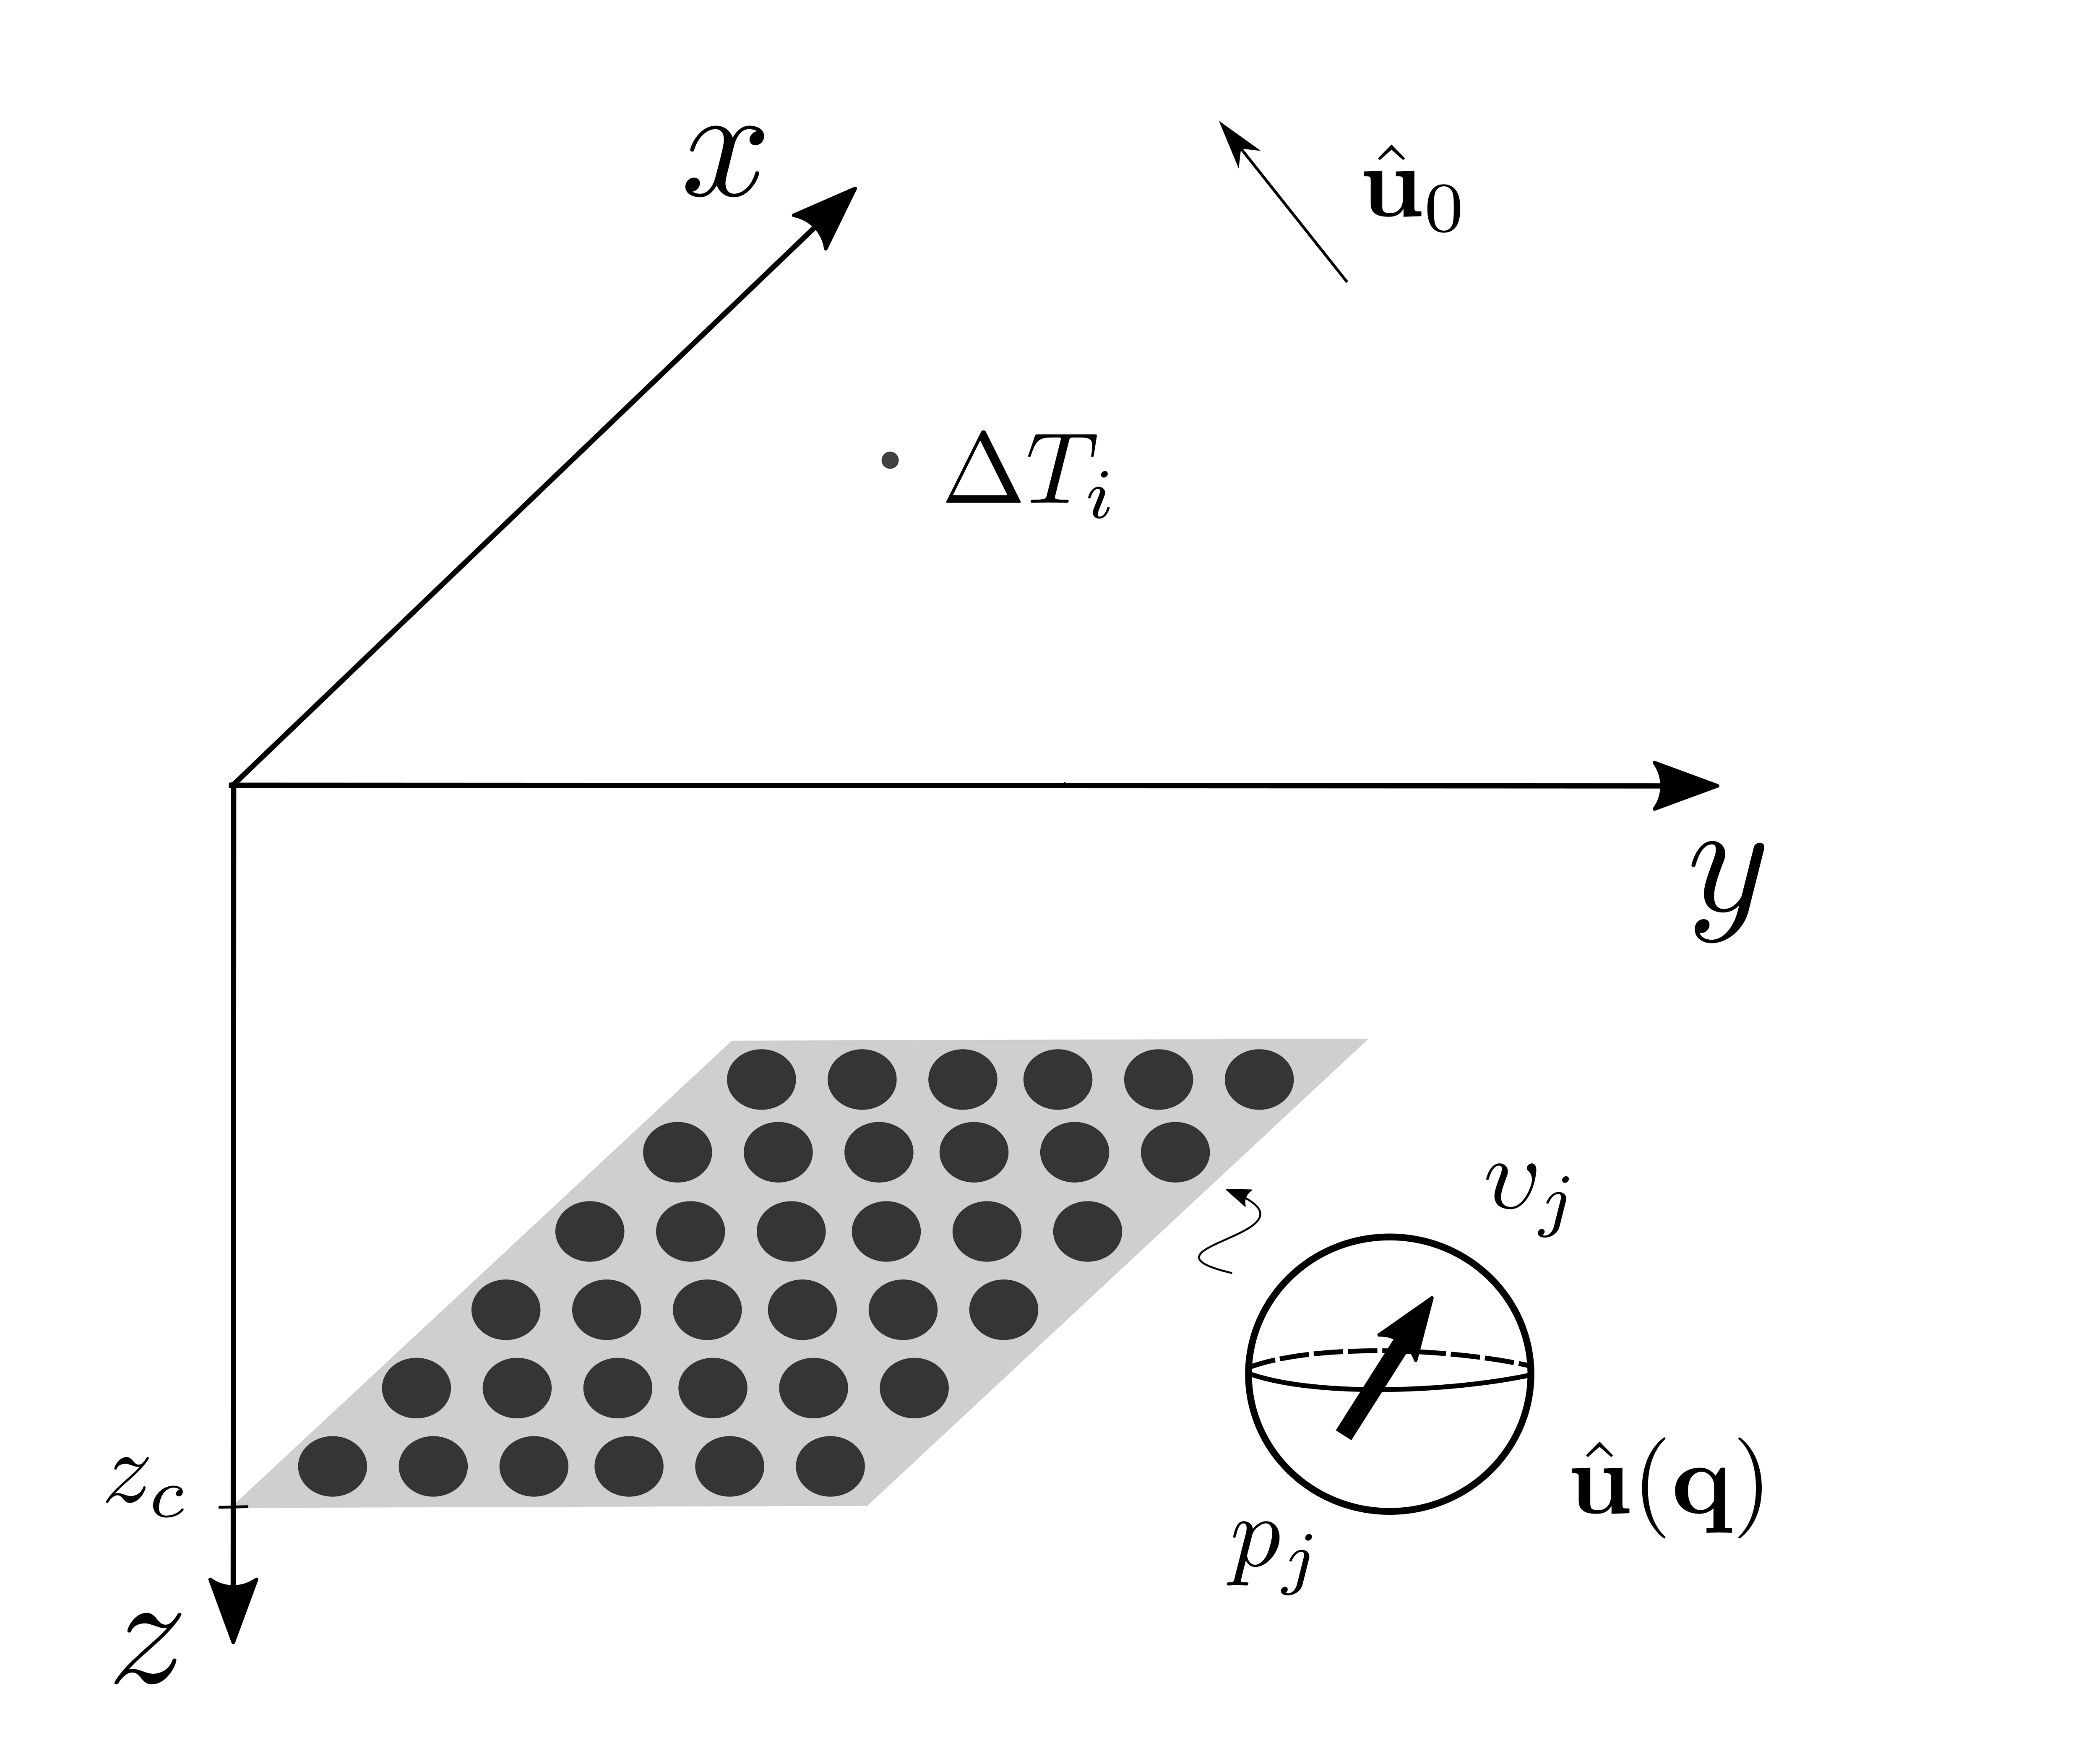
\includegraphics[width=.7\textwidth]{Fig/eqlayer/eqlayer_figure_tfa.png}
	\caption{Representação esquemática da camada equivalente para a anomalia de campo total. A camada é posicionada 
	sobre o plano horizontal a uma profundidade $z=z_{c}$. $\Delta T_{i}(\mathbf{s})$ é a anomalia de campo total predita 
	(equação \ref{eq:tfa-pred-i}) no ponto 
	$(x_{i},y_{i},z_{i})$ produzida pelo conjunto de $M$ fontes equivalentes (pontos pretos). Cada fonte é localizada 
	no ponto  $(x_{j},y_{j},z_{c})$, $j = 1, \dots, M$, e são representadas por um dipolo de volume unitário 
	$\upsilon_{j}$ com direção de magnetização $\hat{\mathbf{u}}(\mathbf{q})$ e momento magnético $p_{j}$. 
	$\hat{\mathbf{u}}_{0} \equiv \hat{\mathbf{u}}(I_{0}, D_{0})$ é um vetor unitário na direção do campo 
	principal.}
	\label{fig:eqlayer_tfa_sketch}
\end{figure}


\subsection{Problema inverso}
\label{subsec:mag_dir_prob_inv}

%%%%% Defining the objective function
Seja $\mathbf{\Delta T}^{o}$ o vetor de dados observados cujo $i$-ésimo elemento é a anomalia de campo 
total produzida, no ponto $(x_{i},y_{i},z_{i})$, $i = 1, \dots, N$, por fontes magnéticas com direção de 
magnetização uniforme. Similarmente, seja $\mathbf{\Delta T} (\mathbf{s})$ o vetor de dados preditos cujo 
$i$-ésimo elemento $\Delta T_{i}(\mathbf{s})$ (equação \ref{eq:tfa-pred-i}) é a anomalia de campo total 
produzida pela camada equivalente discreta no mesmo ponto $(x_{i},y_{i},z_{i})$. 
Para estimar o vetor de parâmetros $\mathbf{s}$ (equação \ref{eq:s-vector}) que minimiza a diferença 
entre $\mathbf{\Delta T}^{o}$ e $\mathbf{\Delta T}(\mathbf{s})$, resolvo o seguinte problema inverso:
\begin{subequations}
	\begin{align}
	& \text{minimizar}
	& &\Psi(\mathbf{s}) =\lVert \mathbf{\Delta T}^{o} - \mathbf{\Delta T} (\mathbf{s}) 
	\rVert_{2}^{2} + \, \mu f_0 \parallel \mathbf{p} \parallel_{2}^{2} \: , \\
	& \text{sujeito a}
	& & p_{j} \geqslant 0 \: , \quad j = 1, \dots, M \: .
	\end{align}
	\label{eq:positivity_goal_function}
\end{subequations}
O primeiro e o segundo termo da equação \ref{eq:positivity_goal_function}a são, respectivamente, a função de ajuste e a função 
regularizadora de Tikhonov de ordem zero, $\mu$ é o parâmetro de regularização, $\| \cdot \|_{2}^{2}$ representa o quadrado da 
norma Euclidiana e $f_{0}$ é um fator de normalização. A equação \ref{eq:positivity_goal_function}b impõe que todos os elementos 
$p_{j}$ do vetor de momentos magnéticos $\mathbf{p}$ sejam maiores ou iguais a zero. 
Este vínculo de positividade se baseia no resultado teórico deduzido na seção \ref{sec:distribuicao-positiva} e 
é incorporado utilizando o \textit{estimador de mínimos quadrados não negativo}, ou NNLS 
(do inglês \textit{Nonnegative least squares}), proposto por \citep{lawson_hanson_1974}.

Para resolver este problema inverso, considere uma expansão até segunda ordem da função $\Psi(\mathbf{s})$
(equação \ref{eq:positivity_goal_function}a) em torno de $\mathbf{s} = \mathbf{s}^{k}$ 
(equação \ref{eq:s-vector}):
\begin{equation}
\Psi(\mathbf{s}^{k} + \mathbf{\Delta s}^{k}) \approx \Psi(\mathbf{s}^{k}) + 
{\mathbf{J}^{k}}^{\top} \mathbf{\Delta s}^{k} + 
\frac{1}{2} {\mathbf{\Delta s}^{k}}^{\top} \mathbf{H}^{k} \mathbf{\Delta s}^{k}  \: ,
\label{eq:sec_ord_goal}
\end{equation}
em que $\mathbf{\Delta s}^{k}$ é uma perturbação no vetor de parâmetros $\mathbf{s}$ 
(equação \ref{eq:s-vector}) e os termos 
$\mathbf{J}^{k}$ e $\mathbf{H}^{k}$ são, respectivamente, o vetor gradiente e a matriz Hessiana avaliadas em $\mathbf{s}^{k}$. 
Calculando o gradiente do lado direito da equação \ref{eq:sec_ord_goal} em relação a $\bar{\mathbf{\Delta s}}^{k}$
e igualando o resultado ao vetor nulo, deduzimos o seguinte sistema linear:
\begin{equation}
\mathbf{H}^{k} \bar{\mathbf{\Delta s}}^{k} = - \mathbf{J}^{k} \: ,
\label{eq:linear_sys_GN}
\end{equation}
que representa o $k$-ésimo passo do método de Gauss-Newton \citep{aster2005} para a minimização da função objetivo (equação \ref{eq:positivity_goal_function}a). Reescrevemos este sistema linear desprezando as derivadas cruzadas na matriz Hessiana como: 
\begin{equation}
\left[
\begin{array}{c|c}
\mathbf{H}_{pp}^{k} & \mathbf{0} \\
\hline
\mathbf{0}^{\top} & \mathbf{H}_{qq}^{k}
\end{array}
\right] \left[ \begin{array}{c}
\bar{\mathbf{\Delta p}}^{k} \\ 
\bar{\mathbf{\Delta q}}^{k} 
\end{array} \right] \approx -\left[ \begin{array}{c}
\mathbf{J}_{p}^{k} \\ 
\mathbf{J}_{q}^{k} 
\end{array} \right] ,
\label{eq:linear_sys_GN_block}
\end{equation}
em que $\mathbf{0}$ é uma matriz $M \times 2$ que contém todos os elementos iguais a zero, 
$\bar{\mathbf{\Delta p}}^{k} = \bar{\mathbf{p}}^{k+1} - \bar{\mathbf{p}}^{k}$ é a correção no vetor de momentos magnéticos 
$\mathbf{p}$, $\bar{\mathbf{\Delta q}}^{k} = \bar{\mathbf{q}}^{k+1} - \bar{\mathbf{q}}^{k}$ é a correção no vetor direção 
de magnetização $\mathbf{q}$ e os termos $\mathbf{J}_{\alpha}^{k}$ e $\mathbf{H}_{\alpha \alpha}^{k}$, $\alpha = p,q$, 
são os vetores gradientes e as matrizes Hessianas calculadas com relação aos elementos de $\mathbf{p}$ e $\mathbf{q}$, 
respectivamente. 

O vetor gradiente $\mathbf{J}_{p}^{k}$ e a matriz Hessiana $\mathbf{H}_{pp}^{k}$ (equação \ref{eq:linear_sys_GN_block}) 
relativos ao vetor de momentos magnéticos $\mathbf{p}$ são, respectivamente, 
\begin{equation}
\mathbf{J}_{p}^{k} = -2 {\mathbf{G}_{p}^{k}}^{\top} 
\left[ \mathbf{\Delta T}^{o} - \mathbf{\Delta T} (\bar{\mathbf{s}}^{k}) \right] + 
2\mu f_{0}^{k} \bar{\mathbf{p}}^{k} 
\label{eq:grad_p}
\end{equation}
e 
\begin{equation}
\mathbf{H}_{pp}^{k} = 2 {\mathbf{G}_{p}^{k}}^{\top} \mathbf{G}_{p}^{k} + 
2 \mu f_{0}^{k} \mathbf{I} \: ,
\label{eq:hess_p}
\end{equation}
em que $\mathbf{G}_p^{k}$ é uma matriz $N \times M$ cujo elemento $ij$ é definido pela função 
harmônica $g_{ij}(\bar{\mathbf{q}}^{k})$ (equação \ref{eq:g_ij}) avaliada na direção de magnetização 
$\bar{\mathbf{q}}^{k}$, $\mathbf{I}$ é a matriz identidade $M \times M$ e $f_{0}^{k}$ é um fator de 
normalização igual a 
\begin{equation}
f_{0}^{k} = \dfrac{trace \left({\mathbf{G}_{p}^{k}}^{\top} \mathbf{G}_{p}^{k} \right)}{M} \, .
\label{eq:norm_factor}
\end{equation}
O vetor gradiente $\mathbf{J}_{q}^{k}$ e a matriz Hessiana $\mathbf{H}_{qq}^{k}$ (equação \ref{eq:linear_sys_GN_block}) 
relativos a direção de magnetização $\mathbf{q}$ são, respectivamente, 
\begin{equation}
\mathbf{J}_{q}^{k} = -2 {\mathbf{G}_{q}^{k}}^{\top} 
\left[ \mathbf{\Delta T}^{o} - \mathbf{\Delta T} (\bar{\mathbf{s}}^{k}) \right]
\label{eq:grad_q}
\end{equation}
e
\begin{equation}
\mathbf{H}_{qq}^{k} \approx 2 {\mathbf{G}_{q}^{k}}{^\top} \mathbf{G}_{q}^{k} \: ,
\label{eq:hess_q}
\end{equation}
em que $\mathbf{G}_{q}^{k}$ é uma matriz $N \times 2$ dada por 
\begin{equation}
\mathbf{G}_{q}^{k} = \begin{bmatrix}
\partial_{I} \mathbf{g}_{1}(\bar{\mathbf{q}}^{k})^{\top} \bar{\mathbf{p}}^{k} & 
\partial_{D} \mathbf{g}_{1}(\bar{\mathbf{q}}^{k})^{\top} \bar{\mathbf{p}}^{k} \\
\vdots & \vdots  \\
\partial_{I} \mathbf{g}_{N}(\bar{\mathbf{q}}^{k})^{\top} \bar{\mathbf{p}}^{k} & 
\partial_{D} \mathbf{g}_{N}(\bar{\mathbf{q}}^{k})^{\top} \bar{\mathbf{p}}^{k} 
\end{bmatrix} \: ,
\label{eq:Gq}
\end{equation}
e $\partial_{\alpha} \mathbf{g}_{i}(\bar{\mathbf{q}}^{k}) \equiv 
\frac{\partial \mathbf{g}_{i}(\bar{\mathbf{q}}^{k})}{\partial \alpha}$, $\alpha= I, D$, representa a primeira derivada do vetor 
$\mathbf{g}_{i}(\bar{\mathbf{q}}^{k})$ (equação \ref{eq:tfa-pred-i}) com relação a inclinação $I$ e a declinação $D$ 
da magnetização das fontes equivalentes.

\subsection{Processo iterativo para a estimativa da direção de magnetização}
\label{subsec:iterative-proccess}

Na iteração $k=0$, utilizamos uma aproximação inicial $\bar{\mathbf{q}}^{k} = \bar{\mathbf{q}}^{0}$ 
para o vetor direção de magnetização $\mathbf{q}$ (equação \ref{eq:q-vector}) e, manipulando a 
parte superior da equação \ref{eq:linear_sys_GN_block}, definimos o seguinte sistema linear 
para o vetor de momentos magnéticos $\mathbf{p}$:
\begin{equation}
\left[ {\mathbf{G}_{p}^{k}}^{\top} \mathbf{G}_{p}^{k} + 
\mu f_{0}^{k} \, \mathbf{I} \right] \bar{\mathbf{p}}^{k} = 
{\mathbf{G}_{p}^{k}}^{\top} \mathbf{\Delta T}^{o} \: .
\label{eq:linear_sys_p}
\end{equation}
Para impor o vínculo de positividade (equação \ref{eq:positivity_goal_function}b) ao vetor $\mathbf{p}$, este sistema 
linear (equação \ref{eq:linear_sys_p}) é resolvido usando o método de NNLS \citep{lawson_hanson_1974, silvadias_etal_2007}. 
Esta distribuição de momentos magnéticos é então usada para estimar uma correção $\bar{\mathbf{\Delta q}}^{k}$ no vetor 
direção de magnetização resolvendo o seguinte sistema não-linear via método de Levenberg-Marquardt 
\citep{aster2005}:
\begin{equation}
\left[ {\mathbf{G}_{q}^{k}}^{\top} \mathbf{G}_{q}^{k} + \lambda \, \mathbf{I} \right] 
\bar{\mathbf{\Delta q}}^{k} = {\mathbf{G}_{q}^{k}}^{\top} 
\left[ \mathbf{\Delta T}^{o} - \mathbf{\Delta T} (\mathbf{s}^{k}) \right] \: ,
\label{eq:linear_sys_q}
\end{equation}
em que $\lambda$ é o parâmetro de Marquardt e $\mathbf{I}$ é uma matriz identidade. Após estimarmos a correção 
$\bar{\mathbf{\Delta q}}^{k}$ na $k$-ésima iteração, atualizamos a direção de magnetização 
aplicando a correção abaixo:
\begin{equation}
\bar{\mathbf{q}}^{k+1} = \bar{\mathbf{q}}^{k} + \bar{\mathbf{\Delta q}}^{k} \: .
\label{eq:q_next}
\end{equation}
O vetor $\bar{\mathbf{q}}^{k+1}$ é usado para estimar uma nova distribuição de momentos magnéticos com a equação 
\ref{eq:linear_sys_p} e assim sucessivamente. O processo iterativo é interrompido quando a função objetivo 
(equação \ref{eq:positivity_goal_function}a) é invariante ao longo de sucessivas iterações. Neste 
caso, espera-se que a camada equivalente reproduza os dados de anomalia de campo total e 
que sua direção de magnetização seja próxima a das fontes verdadeiras.

\subsection{Limitação para o caso de fontes magnetizadas verticalmente}
\label{subsec:vertical-magnetization}

O método descrito na subseção \ref{subsec:iterative-proccess} falha quando a magnetização total das 
fontes possui a direção igual ou aproximadamente vertical. A seguir, apresento a base teórica para o 
entendimento desta limitação. 

Considere o caso limite no qual a magnetização total das fontes é vertical e.g., $I = \pm 90^\circ$). 
Neste caso, a anomalia de campo total $\Delta T(x, y, z)$ (equação \ref{eq:Delta-T-true-mag-uniform}) 
não depende da declinação $D$. Isso pode ser deduzido a partir das equações \ref{eq:u-hat} e 
\ref{eq:a-coefficients-sources} e mostra o seguinte fato: fontes magnetizadas verticalmente não possuem 
uma declinação definida. Consequentemente, em vez de um mínimo bem definido no espaço dos parâmetros, a 
função objetivo $\Psi(\mathbf{s})$ (equação \ref{eq:positivity_goal_function}a) possui uma região de mínimos 
alongada na direção da declinação $D$. Infelizmente, o vínculo de positividade sobre o vetor de momentos magnéticos 
(equação  \ref{eq:positivity_goal_function}b) não resolve esta ambiguidade.

Para entender como esta ambiguidade afeta nosso método, vamos analisar a matriz $\mathbf{G}_{q}^{k}$ 
(equação \ref{eq:Gq}) necessária para estimar a correção $\bar{\mathbf{\Delta q}}^{k}$ para a direção de 
magnetização (equação \ref{eq:linear_sys_q}). Sua $i$-ésima linha é definida como o produto do vetor de momentos magnéticos 
estimado $\bar{\mathbf{p}}^{k}$ e as primeiras derivadas $\partial_{\alpha} \mathbf{g}_{i}(\bar{\mathbf{q}}^{k})$, $\alpha= I, D$, 
do vetor $\mathbf{g}_{i}(\mathbf{q})$ (equação \ref{eq:tfa-pred-i}), avaliadas em $\mathbf{q} = \bar{\mathbf{q}}^{k}$, com relação 
a inclinação $I$ e a declinação $D$ das fontes equivalentes. O $j$-ésimo elemento $\partial_{\alpha} g_{ij}(\bar{\mathbf{q}}^{k})$ 
do vetor $\partial_{\alpha} \mathbf{g}_{i}(\bar{\mathbf{q}}^{k})$ é dado por
\begin{equation}
\partial_{\alpha} g_{ij}(\bar{\mathbf{q}}^{k}) = 
\gamma_{m}  \hat{\mathbf{F}}_{0}^T \, \mathbf{M}_{ij} 
\partial_{\alpha} \hat{\mathbf{u}}(\bar{\mathbf{q}}^{k}) \: , \quad \alpha = I, D \: ,
\label{eq:D-alpha-gij}
\end{equation}
em que 
\begin{equation}
\partial_{I} \hat{\mathbf{u}}(\bar{\mathbf{q}}^{k}) = 
\begin{bmatrix}
	-\sin \bar{I}^{k} \cos \bar{D}^{k} \\
	-\sin \bar{I}^{k} \sin \bar{D}^{k} \\
	 \cos \bar{I}^{k}
\end{bmatrix}
\label{eq:D_mag_vec_inc}
\end{equation}
e 
\begin{equation}
\partial_{D} \hat{\mathbf{u}}(\bar{\mathbf{q}}^{k}) = 
\begin{bmatrix}
	-\cos \bar{I}^{k} \sin \bar{D}^{k} \\
	 \cos \bar{I}^{k} \cos \bar{D}^{k} \\
	 0
\end{bmatrix}
\label{eq:D_mag_vec_dec}
\end{equation}
são as derivadas do vetor unitário $\hat{\mathbf{u}}(\mathbf{q}) \equiv \hat{\mathbf{u}}(I, D)$ (equação \ref{eq:u-hat})
com relação a $I$ e $D$, avaliadas na direção de magnetização 
$\bar{\mathbf{q}}^{k} = \left[ \bar{I}^{k} \:\: \bar{D}^{k} \right]^{\top}$. 
 
Note que, quando a inclinação estimada $\bar{I}^{k}$ se aproxima de $\pm 90^{\circ}$, todos os elementos que formam o vetor 
$\partial_{D} \hat{\mathbf{u}}(\bar{\mathbf{q}}^{k})$ (equação \ref{eq:D_mag_vec_dec}) e, consequentemente, a segunda coluna 
da matriz $\mathbf{G}_{q}^{k}$ (equação \ref{eq:Gq}) tendem a zero. Como consequência, o problema não-linear para estimar a 
direção de magnetização (equação \ref{eq:linear_sys_q}) torna-se insensível a mudanças na declinação $D$ e a convergência 
do método fica muito lenta. 


\section{Profundidade da camada ($\mathbf{z_{c}}$) e parâmetro de regularização ($\mathbf{\mu}$)}

Nos métodos descritos nas seções \ref{sec:componentes_campo} e \ref{sec:mag_dir_est}, 
dois parâmetros são importantes. O primeiro é a profundidade da camada $z_{c}$ (Figuras \ref{fig:eqlayer_tfa_sketch} e 
\ref{fig:eqlayer_balpha_sketch}) e o segundo é o parâmetro de regularização $\mu$ 
(equações \ref{eq:goal_function_vec} e \ref{eq:positivity_goal_function}a). 

O método utilizado para a escolha da profundidade da camada é baseado na abordagem clássica proposta por 
\cite{dampney1969}. Aquele autor aponta que a distância relativa entre os planos da camada e dos dados 
observados deve variar entre $2,5$ a $6,0$ vezes o espaçamento do grid de dados. Vale ressaltar que 
\cite{dampney1969} aplicou este criério de escolha a da profundidade da camada usando dados gravimétricos 
regularmente espaçados. No presente trabalho, adaptei o critério de \cite{dampney1969} e defini que a 
distância relativa da camada até a altitude média dos dados deve variar entre $2$ a $3$ vezes o valor do 
maior espaçamento entre os dados. É necessário ressaltar que este intervalo foi definido empiricamente. 

Já para determinar o parâmetro de regularização $\mu$ (equações \ref{eq:goal_function_vec} e 
\ref{eq:positivity_goal_function}a), usei o método da curva-L \citep{hansen-oleary1993}, que serve como 
uma filtragem de ruídos dos dados, sem que o resultado final perca informações. O ``cotovelo" desta curva é 
o valor ótimo de parâmetro no qual é feito o balanço entre a função de ajuste e a função regularizadora. 